\documentclass[../../main/main.tex]{subfiles}
\graphicspath{{./figures/}}

\dominitoc
\faketableofcontents

\renewcommand{\mtcSfont}{\small\bfseries}
\renewcommand{\mtcSSfont}{\footnotesize}
\mtcsettitle{minitoc}{}
\mtcsetrules{*}{off}

\makeatletter
\renewcommand{\@chapapp}{Thermodynamique -- chapitre}
\makeatother

% \toggletrue{student}
% \toggletrue{corrige}
% \renewcommand{\mycol}{black}
% \renewcommand{\mycol}{gray}

\hfuzz=5.002pt

\begin{document}
\setcounter{chapter}{0}

\settype{book}
\settype{prof}
\settype{stud}

\chapter{Description d'un système à l'équilibre}

% \vspace*{\fill}

\begin{tcn}*(ror)<ctc>{\iconsomm~Sommaire}
	\vspace{-15pt}
	\minitoc
	\vspace{-25pt}
\end{tcn}

% \vspace*{\fill}
% \begin{prgm}
% \small
% \begin{tcn}*(ror)"know"{Savoirs}
% 	\begin{itemize}
% 		\item Principe de construction, lecture et utilisation d'un diagramme
% 		      potentiel-pH.
% 		\item Diagramme potentiel-pH de l'eau.
% 	\end{itemize}
% \end{tcn}
\begin{tcn}*[sidebyside, sidebyside align=top](ror)<ctc>""{\iconhow~Capacités exigibles}
	\small
	\begin{itemize}[label=\rcheck]
		\item Définir l'échelle mésoscopique et en expliquer la nécessité.
		\item Citer quelques ordres de grandeur de libres parcours moyens.
		\item Préciser les paramètres nécessaires à la description d'un état
		      microscopique et d'un état macroscopique sur un exemple.
		\item Calculer l'ordre de grandeur d'une vitesse quadratique moyenne dans un
		      gaz parfait.
		\item Identifier un système ouvert, un système fermé, un système isolé.
		\item Calculer une pression à partir d'une condition d'équilibre mécanique.
		\item Déduire une température d'une condition d'équilibre thermique.
		\item Citer et utiliser l'équation d'état des gaz parfaits.
	\end{itemize}
	\tcblower
	\begin{itemize}[label=\rcheck]
		\item Citer quelques ordres de grandeur de volumes molaires ou massiques
		      dans les conditions usuelles de pression et de température.
		\item Exprimer l'énergie interne d'un gaz parfait monoatomique à partir de
		      l'interprétation microscopique de la température.
		\item Exploiter la propriété $U_m = U_m(T)$ pour un gaz parfait, d'une part,
		      et une phase incompressible et indilatable d'autre part.
		\item Interpréter graphiquement la différence de compressibilité entre un
		      liquide et un gaz à partir d'isothermes expérimentales.
		\item Comparer le comportement d'un gaz réel au modèle du gaz parfait sur
		      des réseaux d'isothermes expérimentales en coordonnées de
		      \textsc{Clapeyron} ou d'\textsc{Amagat}.
		      % \item Analyser un diagramme de phase expérimental $(P,T)$.
		      % \item Proposer un jeu de variables d'état suffisant pour caractériser l'état
		      %       d'équilibre d'un corps pur diphasé soumis aux seules forces de pression.
		      % \item Positionner les phases dans les diagrammes $(P,T)$ et $(P,v)$.
		      % \item Déterminer la composition d'un mélangé diphasé en un point d'un
		      %       diagramme $(P,v)$.
	\end{itemize}
\end{tcn}
% \end{prgm}
\vspace{-15pt}

% \vspace*{\fill}

\newpage

\vspace*{\fill}
% {
% \begin{boxes}
\begin{tcn}*[sidebyside](ror)<ctc>{\iconchek~L'essentiel}
	\small
	\begin{tcn}*(defi)<ctc>{\icondefi~Définitions}
		\tcblistof[\paragraph*]{defi}{\hspace*{4.8pt}}
	\end{tcn}
	% \begin{tcn}(rapp)<ctc>{Rappels}
	%   \tcblistof[\paragraph*]{rapp}{\hspace*{4.8pt}}
	% \end{tcn}
	\begin{tcn}*(prop)<ctc>{\iconprop~Propriétés}
		\tcblistof[\paragraph*]{prop}{\hspace*{4.8pt}}
		\tcblistof[\paragraph*]{loi}{\hspace*{4.8pt}}
		% \tcblistof[\paragraph*]{theo}{\hspace*{4.8pt}}
	\end{tcn}
	% \begin{tcn}*(coro)<ctc>{Corollaires}
	%   \tcblistof[\paragraph*]{coro}{\hspace*{4.8pt}}
	% \end{tcn}
	% \begin{tcn}*(demo)<ctc>{Démonstrations}
	%   \tcblistof[\paragraph*]{demo}{\hspace*{4.8pt}}
	%   \tcblistof[\paragraph*]{prev}{\hspace*{4.8pt}}
	% \end{tcn}
	% \begin{tcn}*(inte)<ctc>{Interprétations}
	%   \tcblistof[\paragraph*]{inte}{\hspace*{4.8pt}}
	% \end{tcn}
	% \begin{tcn}*(tool)<ctc>{\icontool~Outils}
	% 	\tcblistof[\paragraph*]{tool}{\hspace*{4.8pt}}
	% \end{tcn}
	% \begin{tcn}*(nota)<ctc>{Notations}
	%   \tcblistof[\paragraph*]{nota}{\hspace*{4.8pt}}
	% \end{tcn}
	% \begin{tcn}*(appl)<ctc>{Applications}
	%   \tcblistof[\paragraph*]{appl}{\hspace*{4.8pt}}
	% \end{tcn}
	% \begin{tcn}*(rema)<ctc>{Remarques}
	%   \tcblistof[\paragraph*]{rema}{\hspace*{4.8pt}}
	% \end{tcn}
	% \begin{tcn}*(exem)<ctc>{Exemples}
	%   \tcblistof[\paragraph*]{exem}{\hspace*{4.8pt}}
	% \end{tcn}
	% \begin{tcn}*(ror)<ctc>{Points importants}
	%   \tcblistof[\paragraph*]{ror}{\hspace*{4.8pt}}
	% \end{tcn}
	% \begin{tcn}*(impo)<ctc>{Erreurs communes}
	%   \tcblistof[\paragraph*]{impo}{\hspace*{4.8pt}}
	% \end{tcn}
	\tcblower
	\small
	% \begin{tcn}*(defi)<ctc>{Définitions}
	%   \tcblistof[\paragraph*]{defi}{\hspace*{4.8pt}}
	% \end{tcn}
	% \begin{tcn}*(rapp)<ctc>{Rappels}
	%   \tcblistof[\paragraph*]{rapp}{\hspace*{4.8pt}}
	% \end{tcn}
	% \begin{tcn}*(prop)<ctc>{Propriétés}
	%   \tcblistof[\paragraph*]{prop}{\hspace*{4.8pt}}
	%   \tcblistof[\paragraph*]{loi}{\hspace*{4.8pt}}
	%   \tcblistof[\paragraph*]{theo}{\hspace*{4.8pt}}
	% \end{tcn}
	% \begin{tcn}*(coro)<ctc>{Corollaires}
	%   \tcblistof[\paragraph*]{coro}{\hspace*{4.8pt}}
	% \end{tcn}
	\begin{tcn}*(demo)<ctc>{Démonstrations}
		\tcblistof[\paragraph*]{demo}{\hspace*{4.8pt}}
		\tcblistof[\paragraph*]{prev}{\hspace*{4.8pt}}
	\end{tcn}
	\begin{tcn}*(inte)<ctc>{Interprétations}
		\tcblistof[\paragraph*]{inte}{\hspace*{4.8pt}}
	\end{tcn}
	% \begin{tcn}*(tool)<ctc>{Outils}
	%   \tcblistof[\paragraph*]{tool}{\hspace*{4.8pt}}
	% \end{tcn}
	% \begin{tcn}*(nota)<ctc>{Notations}
	%   \tcblistof[\paragraph*]{nota}{\hspace*{4.8pt}}
	% \end{tcn}
	\begin{tcn}*(appl)<ctc>{\iconappl~Applications}
		\tcblistof[\paragraph*]{appl}{\hspace*{4.8pt}}
	\end{tcn}
	% \begin{tcn}*(rema)<ctc>{Remarques}
	%   \tcblistof[\paragraph*]{rema}{\hspace*{4.8pt}}
	% \end{tcn}
	% \begin{tcn}*(exem)<ctc>{Exemples}
	% 	\tcblistof[\paragraph*]{exem}{\hspace*{4.8pt}}
	% \end{tcn}
	\begin{tcn}*(ror)<ctc>{\iconhart~Points importants}
		\tcblistof[\paragraph*]{ror}{\hspace*{4.8pt}}
	\end{tcn}
	\begin{tcn}*(impo)<ctc>{\iconimpo~Erreurs communes}
		\tcblistof[\paragraph*]{impo}{\hspace*{4.8pt}}
	\end{tcn}
\end{tcn}
% \end{boxes}
% }%

\vspace*{\fill}
\newpage

% Comme son nom l'indique, la thermo/dynamique est le domaine de la physique qui
% s'intéresse au lien entre les aspects thermiques (le «~chaud~» et le «~froid~»)
% et le mouvement. C'est son émergence entre la fin du \textsc{xviii}\ieme{} et le
% début du \textsc{xix}\ieme{} siècle qui a permis la révolution industrielle,
% dont la «~machine à vapeur~» est emblématique.
% \bigbreak
% Aujourd'hui encore, le fonctionnement de multiples systèmes exploite les lois de
% la thermodynamique. Citons par exemple les réfrigérateurs ou les moteurs des
% voitures à essence. La production d'électricité dans une centrale thermique,
% qu'elle soit nucléaire, géothermique ou à charbon, commence également par une
% conversion d'énergie thermique en énergie mécanique, avant que cette énergie
% mécanique ne soit convertie en énergie électrique grâce aux phénomènes
% d'induction.

\section{Introduction}
La thermodynamique s'intéresse fondamentalement à des systèmes à taille humaine,
contenant un grand nombre de particules. Pour passer de nombres aux quantités de
matière, on utilise le \textbf{nombre d'\textsc{Avogadro}} qui définit la mole~:

\begin{tcb}[sidebyside](defi){Nombre d'\textsc{Avogadro}}
	La quantité de matière d'un système se note $n$ et se définit par
	\psw{
		\[
			\boxed{n = \frac{N}{\Nc_A}}
			\quad \text{en \textbf{moles}, \si{mol}}
		\]
	}%
	\tcblower
	avec $N$ le nombre d'entités dans l'échantillon, et $\Nc_A$ est une
	constante nommée \textbf{nombre d'\textsc{Avogadro}} telle que
	\psw{
		\[
			\Nc_A = \SI{6.02214076e23}{mol^{-1}}
		\]
	}%
\end{tcb}

\subsection{Quelques ordres de grandeur}
\begin{tcb}(odgr)<lftt>{Molécules de quelques systèmes}
	Estimez le nombre de molécules dans~:
	\begin{tasks}[label=\arabic*)](2)
		\task Un verre d'eau~;
		\task La salle de classe.
	\end{tasks}
	\tcblower
	\begin{enumerate}
		\item \psw{
			      Soit $m\ind{eau} \approx \SI{200}{g}$ et $M(\ce{H_2O}) = \SI{18}{g.mol^{-1}}$~:
			      \[
				      n = \frac{m}{M} = \SI{11}{mol}
				      \qso
				      N = n \Nc_A = \SI{6.7e24}{molécules d'eau}
			      \]
		      }%
		\item \psw{%
			      Surface $S = \SI{50}{m^2}$ et hauteur $h = \SI{3.0}{m}$ donc volume
			      $V = \SI{150}{m^3}$~; avec $\th = \SI{20}{\degreeCelsius} \Lra T =
				      \SI{293}{K}$ et $P = \SI{1}{bar} = \SI{e5}{Pa}$, soit avec la loi
			      du gaz parfait
			      \[
				      n = \frac{PV}{RT} \approx \SI{6e3}{mol}
				      \qso
				      N = n \Nc_A = \SI{3.7e27}{molécules}
			      \]
		      }%
	\end{enumerate}
\end{tcb}

\begin{tcb}(inte){Nécessité de la thermodynamique}
	Il y a un nombre bien trop élevé de particules à étudier~! Même les meilleures
	simulations de dynamique n'atteignent que \SI{e12}{molécules}~: il faudrait
	dix millions de millions d'ordinateurs superpuissants pour décrire un litre
	d'eau.
	\smallbreak
	De plus, seule une infime fraction de cette information est réellement
	intéressante~: on ne veut que quelques critères pour décrire et quantifier des
	phénomènes (changements d'état, transferts thermiques…)
\end{tcb}

\subsection{Échelles de description d'un fluide}

Selon la taille du système étudié, on voit la matière avec un point de vue
\textbf{continu}, où la matière est décrit par son comportement global (par
exemple la mécanique), ou \textbf{discontinu} (ou \textbf{discret}), où la
matière est vue comme la somme de ses constituants élémentaires (par exemple
l'architecture de la matière). Ceci est caractérisé par la \textbf{distance
	entre les molécules}~:
\begin{tcb}(odgr)<lftt>{Distances intermoléculaires}
	À pression et température normales~:
	\begin{itemize}
		\bitem{Dans un liquide ou un solide}~:
		\psw{$d \approx \SI{e-10}{m}$}
		\bitem{Dans un gaz}~:
		\psw{$d \approx \SIrange{e-8}{e-7}{m}$}
	\end{itemize}
\end{tcb}

Une autre manière de la décrire est le \textbf{libre parcours moyen}~:
\begin{tcb}(defi){Libre parcours moyen}
	\noindent
	\begin{minipage}[c]{.75\linewidth}
		Le \textbf{libre parcours moyen} d'une particule, noté $\ell^*$, est la
		distance moyenne qu'elle parcourt entre \textbf{deux collisions successives}.
	\end{minipage}
	\hfill
	\begin{minipage}[c]{.23\linewidth}
		\vspace{0pt}
		\begin{center}
			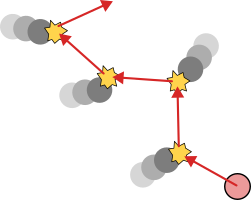
\includegraphics[width=\linewidth]{lbr_prcs}
		\end{center}
	\end{minipage}
\end{tcb}
\begin{tcb}(odgr)<lftt>{Libre parcourt moyen}
	Dans un gaz, $\ell^* \approx \SI{0.1}{\micro m}$~; dans un liquide, $\ell^*
		\approx \SI{1}{nm}$.
\end{tcb}

\begin{tcb*}(defi){Échelles de description}
	Un système peut avoir des comportements très différents suivant sa taille
	caractéristique, appelée \textbf{échelle}. On distingue deux extrêmes~:
	\begin{itemize}
		\bitem{Microscopique}~: celle des particules élémentaires du système, de
		l'ordre de \xul{\psw{\SI{e-10}{m}}}. À cette échelle, la matière est
		discontinue, et caractérisée par une collection de positions et de vitesses
		individuelles.
		\bitem{Macroscopique}~: c'est notre échelle, d'ordre de grandeur de
		\xul{\psw{\SI{1}{m}}}. La matière paraît continue, et peut être décrite par
		des \textbf{paramètres d'état} (voir plus loin).
	\end{itemize}
	On introduit entre les deux une nouvelle échelle~:
	\begin{itemize}
		\bitem{Mésoscopique}~: c'est l'échelle intermédiaire, de l'ordre de
		\xul{\psw{\SI{10}{\micro m}}}. Elle est~:
		\begin{itemize}
			\bitem{Ni trop petite}~: elle contient un grand nombre de particules et on
			peut y définir des \textbf{valeurs moyennes}~;
			\bitem{Ni trop grande}~: elle est quasi-ponctuelle à l'échelle
			macroscopique pour rendre compte des \textbf{inhomogénéités} des
			paramètres d'état.
		\end{itemize}
	\end{itemize}
\end{tcb*}

\begin{tcb}(appl)<lftt>{Échelles}
	Déterminer pour la salle de cours un volume macroscopique, microscopique et
	enfin mésoscopique.
	\tcblower
	\begin{itemize}
		\bitem{Macroscopique}~:
		\psw{%
			L'ensemble de la salle, soit \SI{240}{m^3}
		}%
		\bitem{Microscopique}~:
		\psw{%
			Cube de côté \SI{0.1}{\micro m}
		}%
		\bitem{Mésoscopique}~:
		\psw{%
			Cube de côté \SI{1}{mm}
		}%
	\end{itemize}
\end{tcb}
\begin{tcb}[breakable](exem)<lftt>{Radiateur}
	Le chauffage d'une classe en hiver constitue un exemple de situation où une
	modélisation à l'échelle mésoscopique est intéressante. La température n'est
	pas uniforme dans toute la classe : vous savez très bien qu'il fait plus chaud
	près du radiateur !
	\bigbreak
	Une modélisation macroscopique ne permet donc pas de décrire comment se
	répartit la température dans la salle. Cependant, il n'est pas non plus
	nécessaire de recourir à une modélisation microscopique et de décrire le
	mouvement de chaque molécule de l'air lorsqu'elle s'approche ou s'éloigne du
	radiateur. Une modélisation où la température est supposée uniforme dans chaque
	volume mésoscopique est la plus adaptée, et conduit à des résultats en
	excellent accord avec l'expérience.
\end{tcb}

% \subsection{Température cinétique d'un gaz}
% Soit un volume mésoscopique, contenant $N \gg 1$ molécules de gaz. Ce qu'on
% appelle \textbf{température} est en fait une mesure de \textbf{l'agitation
% thermique d'un gaz}

\section{Description d'un système}
\subsection{Système thermodynamique}

\begin{tcb*}(defi){Système thermodynamique}
	On appelle \textbf{système thermodynamique} tout système physique constitué
	d'un \textbf{très grand nombre de particules microscopiques}, séparé de
	\textbf{l'extérieur} par une \textbf{surface de contrôle}, matérielle ou
	fictive. Selon le type d'échanges \textit{via} la surface de contrôle, on dit
	qu'il est~:
	\begin{center}
		\begin{tabular}{ccc}
			\toprule
			\textbf{Type} & \textbf{Échange de matière} & \textbf{Échange d'énergie}
			\\
			\midrule
			Ouvert        & \psw{\cmark}                & \psw{\cmark}
			\\
			Fermé         & \psw{\xmark}                & \psw{\cmark}
			\\
			Isolé         & \psw{\xmark}                & \psw{\xmark}
			\\
			\bottomrule
		\end{tabular}
	\end{center}
	% \begin{itemize}
	%   \bitem{Isolé}~: \psw{n'échange ni matière ni énergie~;}
	%   \bitem{Ouvert}~: \psw{échange et matière et énergie~;}
	%   \bitem{Fermé}~: \psw{échange de l'énergie mais pas de matière.}
	% \end{itemize}
\end{tcb*}

\subsection{Grandeurs d'état}
\subsubsection{Définition}

\begin{tcb*}(defi){Grandeur d'état}
	Une \textbf{grandeur d'état} (ou paramètre d'état) est un paramètre qui permet
	de \textbf{caractériser l'état d'un système}.
	\bigbreak
	Seul un petit nombre de grandeurs d'état indépendantes servent à caractériser
	complètement le système~: on les appelle \textbf{variables d'état}. Ainsi, les
	autres grandeurs d'état qui s'en déduisent sont appelées \textbf{fonctions
		d'état}.
\end{tcb*}

\begin{tcb*}(prop){Fonction d'état}
	Une fonction d'état ne dépend \textbf{que de l'état actuel du système},
	\textit{via} les variables d'état~; ainsi, \textbf{elle ne dépend pas du
		chemin suivi}.
\end{tcb*}

\begin{tcb}(exem)<lftt>{Grandeur d'état pour un appartement}
	On prend comme système l'air contenu dans une pièce d'appartement. Pour le
	caractériser totalement, on peut indiquer plusieurs informations~:
	\begin{tasks}[label=\bdmd](2)
		\task \psw{Son volume $V$~;}
		\task \psw{Sa pression $P$~;}
		\task \psw{Sa température $R$~;}
		\task \psw{Sa quantité de matière $n$.}
	\end{tasks}
\end{tcb}

\begin{tcb}(rema)<lftt>{Paramètres micro et mésoscopique}
	Certains paramètres d'état ne correspondent ainsi qu'à une vision
	microscopique, alors que d'autres ne peuvent être définis que sur un
	\textbf{grand nombre de molécules}.
	\begin{itemize}
		\bitem{Paramètres micro}~: \psw{vitesse des molécules, libre parcourt moyen,
			nombre de molécules~;}
		\bitem{Paramètres méso/macro}~: \psw{température, pression, volume, vitesse
			globale.}
	\end{itemize}
\end{tcb}

\subsubsection{Grandeurs intensives et extensives}
\begin{tcb*}(defi){Grandeurs intensives et extensives}
	Soit deux systèmes $\Sigma_1$ et $\Sigma_2$ identiques, avec une grandeur
	d'état $X$ telle que $X_{\Sigma_1} = X_{\Sigma_2}$. Elle est
	dite~:
	\smallbreak
	\begin{isd}
		\tcbsubtitle{\fatbox{\textbf{Extensive}}}
		Elle \psw{est \textbf{proportionnelle} à la quantité de
			matière~:
			\[
				X_{\Sigma_1 + \Sigma_2} = X_{\Sigma_1} + X_{\Sigma_2} = 2 X_{\Sigma_1}
			\]
		}%
		\vspace{-15pt}
		\tcblower
		\tcbsubtitle{\fatbox{\textbf{Intensive}}}
		Elle \psw{elle ne \textbf{dépend pas} de la quantité de
			matière~:
			\[
				X_{\Sigma_1 + \Sigma_2} = X_{\Sigma_1} = X_{\Sigma_2}
			\]
		}%
		\vspace{-15pt}
	\end{isd}
	% \begin{itemize}
	% 	\bitem{Extensive} si \psw{elle est \textbf{proportionnelle} à la quantité de
	% 		matière~:}
	% 	\psw{%
	% 		\[
	% 			X_{\Sigma_1 + \Sigma_2} = X_{\Sigma_1} + X_{\Sigma_2} = 2 X_{\Sigma_1}
	% 		\]
	% 	}%
	% 	\vspace{-15pt}
	% 	\bitem{Intensive} si \psw{elle ne \textbf{dépend pas} de la quantité de
	% 		matière~:}
	% 	\psw{%
	% 		\[
	% 			X_{\Sigma_1 + \Sigma_2} = X_{\Sigma_1} = X_{\Sigma_2}
	% 		\]
	% 	}%
	% 	\vspace{-15pt}
	% \end{itemize}
\end{tcb*}

\begin{tcb}(inte){Grandeurs intensives et extensives}
	En pratique, on retiendra qu'une grandeur \textbf{extensive} caractérise
	l'\textbf{ensemble du système}, alors qu'une grandeur \textit{intensive} peut
	être définie \textit{localement}, en tout point du système
\end{tcb}

\begin{tcb}(exem)<lftt>{Grandeurs intensives et extensives}
	\begin{itemize}
		\bitem{Extensive}~: \psw{masse, volume, charge électrique, énergie}
		\bitem{Intensive}~: \psw{température, pression, masse volumique,
			concentration}
	\end{itemize}
	En ouvrant la porte entre deux pièces, on augmente le volume mais pas la
	température~! On peut définir la température en un point, mais pas le volume
	en un point.
\end{tcb}

\begin{tcb}(rema)<lftt>{}
	Il existe des grandeurs ni intensives ni extensives, par exemple $V^2$ ou
	$\sqrt{m}$, mais elles sont très occasionnelles.
\end{tcb}

\begin{tcb}(defi){Équation d'état}
	Une relation reliant des grandeurs d'état entre elles s'appellent une
	\textbf{équation d'état}, telle qu'il existe une fonction $f$ telle que
	$\boxed{f(\text{var}) = 0}$.
\end{tcb}

Lorsqu'il existe une équation d'état, alors l'une des grandeurs  devient une
fonction d'état, puisqu'elle peut se déduire des trois autres via l'équation
d'état.

\begin{tcb}(exem)<lftt>{Équations d'état}
	\[
		\rho = \psw{\frac{m}{V}}
		\qqet
		c = \psw{\frac{n}{V}}
	\]
\end{tcb}

\begin{tcb*}(defi){Grandeurs massique et molaire}
	À une grandeur extensive $X$, on associe une grandeur~:
	\smallbreak
	\begin{isd}
		\tcbsubtitle{\fatbox{\textbf{Massique $x$}}}
		\psw{%
			\[
				x = \frac{X}{m}
			\]
		}%
		\vspace{-15pt}
		\tcblower
		\tcbsubtitle{\fatbox{\textbf{Molaire $X_m$}}}
		\psw{%
			\[
				X_m = \frac{X}{n}
			\]
		}%
		\vspace{-15pt}
	\end{isd}
	% \begin{itemize}
	% 	\item
	% 	      \leftcenters{%
	% 		      \textbf{massique} $x$~:
	% 	      }{%
	% 		      \psw{$\DS $}
	% 	      }%
	% 	\item
	% 	      \leftcenters{%
	% 		      molaire $X_m$
	% 	      }{%
	% 		      \psw{$\DS X_m = \frac{X}{n}$}
	% 	      }%
	% \end{itemize}
	et les grandeurs $x$ et $X_m$ sont alors \textbf{intensives}.
\end{tcb*}

\begin{tcb*}(odgr)<lftt>{Grandeurs massique et molaire pour l'eau et pour l'air}
	\begin{itemize}
		\item À température et pression ambiantes pour l'eau liquide, de $M(\ce{H_2O}) =
			      \SI{18e-3}{kg.mol^{-1}}$~:
		      \psw{%
		      \[
			      \rho = \SI{1.0e3}{kg.m^{-3}}
			      \qquad
			      v = \frac{V}{m} = \SI{1.0e-3}{m^3.kg^{-1}}
			      \qquad
			      V_m = \frac{V}{n} = \SI{1.8e-3}{L.mol^{-1}}
		      \]
		      }%
		\item À température et pression ambiantes pour l'air, de $M(\text{air}) =
			      \SI{29e-3}{kg.mol^{-1}}$~:
		      \psw{%
		      \[
			      \rho = \SI{1.23}{kg.m^{-3}}
			      \qquad
			      v = \frac{V}{m} = \SI{0.77}{m^3.kg^{-1}}
			      \qquad
			      V_m = \frac{V}{n} = \SI{24}{L.mol^{-1}}
		      \]
		      }%
		      \vspace*{-15pt}
	\end{itemize}
	\vspace*{-15pt}
\end{tcb*}

\subsection{Grandeurs usuelles}
\subsubsection{Température}
Les particules sont constamment en mouvement, même lorsque la matière est
immobile a l'échelle macroscopique~: on parle d'agitation thermique. Il n'y a
pas de mouvement d'ensemble, les mouvements de chaque particules sont
désordonnés.

\begin{tcb}(defi){Température}
	\noindent
	\begin{minipage}[c]{.70\linewidth}
		La \textbf{température} $T$ est une grandeur qui mesure l'\textbf{énergie
			d'agitation thermique} moyenne des particules microscopiques. Elle
		s'exprime en \xul{\psw{kelvins}} de symbole \xul{\psw{K}}
	\end{minipage}
	\hfill
	\begin{minipage}[c]{.27\linewidth}
		\vspace{0pt}
		\begin{center}
			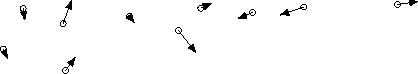
\includegraphics[width=\linewidth]{temp_sch}
			\captionof{figure}{Agitation thermique.}
		\end{center}
	\end{minipage}
\end{tcb}
\begin{tcb}(rema)<lftt>{Température}
	\begin{itemize}
		\item On dit \textbf{kelvin} et non $\cancel{\text{degré kelvin}}$.
		\item On note souvent $\th$ la température en degrés Celsius, tel que
		      \psw{%
			      \[
				      \setlength{\fboxsep}{3mm}
				      \boxed{\th = T - \SI{273.15}{K}}
			      \]
		      }%
		      \vspace*{-15pt}
	\end{itemize}
	\vspace*{-15pt}
\end{tcb}

\subsubsection{Pression}
Lorsque les particules frappent la paroi à cause de l'agitation thermique,
celle-ci subit une force, d'autant plus grande que la surface l'est. La
particule fait alors demi-tour~: elle a donc subi une force dirigée vers
l'intérieur. Par action-réaction, elle a exercé une force dirigée vers
l'\textbf{extérieur}, d'autant plus grande que sa quantité de mouvement l'était.
\begin{tcb*}(defi){Pression}
	\noindent
	\begin{minipage}[c]{.70\linewidth}
		On appelle \textbf{pression} d'un gaz la grandeur physique notée $P$ telle que
		la force $\Ff$ exercée sur une surface $S$ de normale $\nf$ est~:
		\psw{%
			\[
				\setlength{\fboxsep}{3mm}
				\boxed{\Ff = PS \nf}
			\]
		}%
		Son unité est le \xul{\psw{pascal}} de symbole \xul{\psw{Pa}}, tel que
		$\boxed{\psw{\SI{1}{Pa} = \SI{1}{N.m^{-2}}}}$.
	\end{minipage}
	\hfill
	\begin{minipage}[c]{.25\linewidth}
		\vspace{0pt}
		\begin{center}
			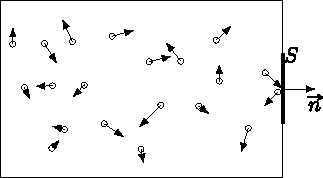
\includegraphics[width=\linewidth]{press_sch}
		\end{center}
	\end{minipage}
\end{tcb*}
\begin{tcb}(rema)<lftt>{Pression}
	Le pascal est une petite unité, on utilise alors souvent le bar qui est la
	pression usuelle~:
	\[
		\setlength{\fboxsep}{3mm}
		\boxed{\psw{\SI{1}{bar} = \SI{e5}{Pa}}}
	\]
\end{tcb}

\subsubsection{Énergie interne}
La thermodynamique permet une nouvelle approche des systèmes, en se basant sur
des études énergétiques plus poussées que nous ne l'avons fait jusque-là en
mécanique. Notamment, on traite les échanges de chaleur avec la thermodynamique.
Il faut pour ça un nouveau «~type~» d'énergie~:

\begin{tcb*}[sidebyside, righthand ratio=.3](defi){Énergie totale}
	L'énergie totale d'un système thermodynamique a deux composantes~:
	\begin{itemize}
		\bitem{\psw{Macroscopique}}~: \psw{c'est l'énergie mécanique $\Ec_m$~;}
		\bitem{\psw{Microscopique}}~: \psw{c'est l'énergie interne $U$.}
	\end{itemize}
	\vspace{-15pt}
	\tcblower
	\[
		\setlength{\fboxsep}{3mm}
		\boxed{\psw{\Ec\ind{tot} = \Ec_m + U}}
	\]
\end{tcb*}

Même en considérant un système macroscopiquement au repos ($\Ec_c = 0$), il a de
l'énergie interne. Une partie de l'énergie interne provient justement du
mouvement microscopique des molécules, traduit par \textbf{l'agitation
	thermique}~: chacune possédant une énergie cinétique, le système total a
nécessairement une contribution cinétique à son énergie interne.
\bigbreak
Le reste de l'énergie provient des \textbf{interactions internes}. On admet
qu'\textbf{elles sont conservatives}, et on y associe donc une énergie
potentielle microscopique. Ainsi,
\begin{tcb*}(defi){Énergie interne}
	L'énergie interne $U$ d'un système est la somme des énergies cinétiques et
	potentielles microscopiques~:
	\psw{%
	\[
		\boxed{U = e_c + e_p}
		\qav
		e_c = \sum_i e_{c,i} = \sum_i \frac{1}{2}m_i v_i{}^2
	\]
	}%
\end{tcb*}

\begin{tcb*}(prop){Énergie interne}
	L'énergie interne est une \textbf{fonction d'état}, et dépend en général de
	$n$, $T$ et $V$~:
	\psw{%
		\[
			\boxed{U = U (n,T,V)}
		\]
	}%
	\vspace{-15pt}
\end{tcb*}

\subsubsection{Capacité thermique}
\begin{tcb*}[label=defi:cv](defi){Capacité thermique à vol.\ constant}
	On appelle \textbf{capacité thermique à volume constant} d'un système fermé la
	grandeur \textbf{extensive}~:
	\psw{%
		\[
			C_V = \pdv{U}{T}
		\]
	}%
	C'est donc la dérivée de l'énergie interne par rapport à la température,
	\textbf{tous les autres paramètres étant constants}.
	\bigbreak
	On définit alors également les capacité thermique \textbf{massique} et
	\textbf{molaire} (intensives) à volume constant~:
	\psw{%
		\[
			c_V = \frac{C_V}{m}
			\qqet
			C_{V,m} = \frac{C_V}{n}
		\]
	}%
\end{tcb*}

\begin{tcb*}(inte){Capacité thermique à vol.\ constant}
	La capacité thermique représente l'aptitude d'un système à absorber ou
	restituer de la chaleur au cours d'une transformation pendant laquelle sa
	température varie.
	\smallbreak
	\begin{isd}[righthand ratio=.4]
		Par exemple, La capacité thermique massique de l'eau est
		\[
			c_{V,\rm eau} = \SI{4.18}{\xul{\psw{kJ.K^{-1}.kg^{-1}}}}
		\]
		Ce qui veut dire que pour élever la température d'une casserole contenant
		$\SI{1}{kg}$ d'eau de $\Delta{T} = \SI{1}{K} = \SI{1}{\degreeCelsius}$, il
		faut apporter une énergie de $\xul{\psw{\SI{4.18}{kJ}}}$.
		\tcblower
		\begin{center}
			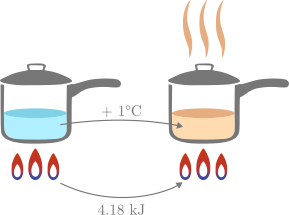
\includegraphics[width=\linewidth]{c_v_eau}
		\end{center}
	\end{isd}
\end{tcb*}

\begin{tcb}(rema)<lftt>{Calorie}
	C'est de là que vient la définition de la calorie~: c'est l'énergie à apporter
	à \SI{1}{g} d'eau liquide sous \SI{1}{bar}, soit $\SI{4.18}{J}$~!
\end{tcb}

\section{Équilibre thermodynamique}
Donner une définition ferme de l'équilibre thermodynamique sans recours à une
théorie plus élaborée (la physique statistique) est loin d'être aisé. Par
conséquent, ce paragraphe donne davantage de caractérisations que de strictes
définitions.

\subsection{Équilibre de systèmes}
Herbet \textsc{Callen}, l'un des fondateurs de la formulation moderne de la
thermodynamique, définit l'équilibre de la manière suivante~:
\begin{center}
	Un système est dit dans un état d'équilibre thermodynamique si son état
	n'évolue pas si il est brusquement isolé de l'environnement extérieur ou coupé
	en deux par une paroi quelle qu'elle soit.
\end{center}
Cette définition est claire sur le plan conceptuel, mais pas la plus utile en
pratique… À notre niveau, il vaut mieux retenir et utiliser une
caractérisation en termes de variables d'état.

\begin{tcb}(defi){Équilibre thermodynamique}
	Un système est dans un état d'\textbf{équilibre thermodynamique} lorsque
	toutes ses \textbf{variables d'état} sont \textbf{uniformes} (dans l'espace)
	et \textbf{constantes} (dans le temps).
\end{tcb}

\begin{tcb*}(impo){Équilibre et isolement}
	\begin{center}
		\fatbox{\textbf{Équilibre $\neq$ isolé}}
	\end{center}
	Un système peut être à l'équilibre tout en continuant à échanger de la matière
	ou de l'énergie avec l'extérieur. Par exemple, l'air contenu dans une pièce
	aérée se renouvelle sans cesse donc c'est un système ouvert, mais la
	température et la pression ne varient pas à l'équilibre.
	\smallbreak
	C'est même \textbf{l'échange permanent} qui permet souvent l'équilibre (sinon
	à 44 personnes dans une salle, elle chauffe~!)
\end{tcb*}

On définira plus loin des équilibres \textbf{instantanés}, où les variables
d'état sont uniformes mais varient dans le temps.

\begin{tcb}(defi){Équilibre entre deux systèmes}
	Deux systèmes sont dits \textbf{en équilibre l'un avec l'autre} si ils sont
	\textbf{individuellement} à l'équilibre et si les échanges d'énergie entre les
	deux systèmes sont terminés ou se compensent.
\end{tcb}

\begin{tcb}(exem)<lftt>{}
	\psw{%
		De l'eau contenu dans un verre posé sur une table depuis longtemps est en
		équilibre thermodynamique avec l'air de la pièce. La température dans l'eau
		et dans l'air est la même, il n'y a donc pas de transfert thermique, et il
		n'y a pas plus d'échange d'énergie mécanique.
	}%
	\begin{center}
		\textbf{Contre-exemples}
	\end{center}
	\psw{%
		Glaçon sorti du congélateur~: température pas constante.
		\bigbreak
		Mur de maison en hiver~: comme la température extérieure n'est pas égale à
		la température dans la maison, la température n'est pas uniforme dans le mur
		et il y a un transfert thermique au travers du mur. Cependant, si la
		différence des températures entre dedans et dehors est constante, la
		répartition de température dans le mur peut ne pas dépendre du temps.
	}%
\end{tcb}

\subsection{Conditions d'équilibres}
\begin{tcb*}(defi){Condition d'équilibre}
	L'équilibre thermodynamique se caractérise par 3 types d'équilibres~:
	\begin{enumerate}
		\bitem{Équilibre physico-chimique}~:
		\psw{%
			sa composition est \textbf{constante} (pas de transformation)~;
		}%
		\bitem{Équilibre thermique}~:
		\psw{%
			sa température est \textbf{uniforme} et \textbf{constante}~;
		}%
		\bitem{Équilibre mécanique}~:
		\psw{%
			pas de mouvement de matière à l'échelle du système
		}%
	\end{enumerate}
\end{tcb*}

\begin{tcb*}(prop){Équilibre thermique}
	Deux systèmes en équilibre thermique l'un avec l'autre n'\textbf{échangent pas
		de chaleur}~; ainsi,
	\begin{center}
		\psw{Deux systèmes en équilibre thermique ont même température~:
			$\boxed{T\ind{syst} = T\ind{ext}}$}
	\end{center}
\end{tcb*}

Déterminer si deux systèmes sont en équilibre mécanique est un peu plus subtil
que pour l'équilibre thermique, et il n'y a pas de critère universel analogue à
l'égalité des températures. Une caractérisation possible passe par l'étude de la
paroi séparant les deux systèmes.

\begin{tcb*}(prop){Équilibre mécanique}
	Deux systèmes sont en équilibre mécanique si et seulement si la paroi les
	séparant est \textbf{immobile}~; autrement dit
	\psw{%
		\[
			\boxed{\sum_i \Ff_{\ext,i}\sup{paroi} = \of}
		\]
	}%
\end{tcb*}

\begin{tcb*}[breakable](appl)<lftt>{Équilibre mécanique}
	Un récipient est séparé de l'extérieur par un piston mobile de masse $m$. On
	appelle $P_0$ la pression extérieure. Déduire de la condition d'équilibre
	mécanique la pression $P_1$ dans le récipient.
	\tcblower
	\noindent
	\begin{minipage}[c]{.78\linewidth}
		\psw{%
			\begin{itemize}
				\bitem{Système} = \{piston\} de masse $m$, $\Rc\ind{labo}$ galiléen et repère
				cartésien, $\uz$ vertical ascendant.
				\bitem{Forces}~: Il subit $\Pf = -mg \uz$, la force de pression de
				l'intérieur $\Ff\ind{int} = P_1S\uz$ et celle de l'extérieur
				$\Ff\ind{ext} = -P_0 S\uz$.
			\end{itemize}
			\begin{gather*}
				\beforetext{\bdmd~Équilibre $\Ra$}
				\sum_i \Ff_{\ext,i} = \of
				\Lra
				P_1S = P_0S + mg
				\\\Lra
				\boxed{P_1 = P_0 + \frac{mg}{S}}
			\end{gather*}
		}%
	\end{minipage}
	\hfill
	\begin{minipage}[c]{.18\linewidth}
		\vspace{0pt}
		\begin{center}
			\sswitch{
				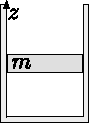
\includegraphics[width=\linewidth]{piston_exo-plain}
			}{
				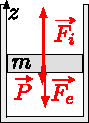
\includegraphics[width=\linewidth]{piston_exo}
			}
			\vspace{-15pt}
			\captionsetup{justification=centering}
			\captionof{figure}{\\Schéma piston.}
		\end{center}
	\end{minipage}
\end{tcb*}

\section{Description d'un gaz}
\subsection{Modélisation}
\begin{tcb*}[breakable](defi){Gaz parfait monoatomique}
	Le modèle du \textbf{gaz parfait monoatomique} implique les hypothèses
	suivantes~:
	\begin{itemize}
		\item \psw{%
			      Il n'est constitué que d'entités à \textbf{un seul atome}~;
		      }%
		\item \psw{%
			      Les atomes sont \textbf{assimilés à des points}~;
		      }%
		\item \psw{%
			      Les atomes sont \textbf{sans interaction} les uns avec les autres.
		      }%
	\end{itemize}
	\begin{isd}
		\begin{center}
			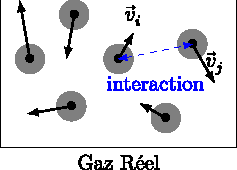
\includegraphics[width=.5\linewidth]{gaz_reel}
			\captionsetup{justification=centering}
			\captionof{figure}{Gaz réel.}
		\end{center}
		\tcblower
		\begin{center}
			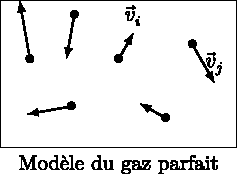
\includegraphics[width=.5\linewidth]{gaz_prft}
			\captionsetup{justification=centering}
			\captionof{figure}{Gaz parfait.}
		\end{center}
	\end{isd}
\end{tcb*}

\begin{tcb}(rema)<lftt>{Gaz parfait}
	\begin{itemize}
		\item Ainsi la nature du gaz (composition chimique des particules le
		      constituant) ne joue aucun rôle. C'est pourquoi rigoureusement il faut
		      parler \textit{du} gaz parfait et non \textit{des} gaz parfaits.

		\item La condition de ponctualité revient à négliger la taille des atomes
		      devant la distance intermoléculaire.

		\item La condition de non-interaction revient à supposer que la distance
		      intermoléculaire est grande devant la distance caractéristique des
		      forces en jeu (principalement celles de \textsc{Van der Waals}).

		\item En pratique, un gaz parfait est un \textbf{gaz dilué} ou bien issu de la
		      famille des gaz nobles (comme l'argon).

		      % \item Le libre parcourt moyen pour un gaz parfait est infini.
	\end{itemize}
\end{tcb}
\vspace{-15pt}

\subsection{Équation d'état}
\subsubsection{Gaz parfait}

À l'équilibre thermodynamique, les variables d'état $P$, $V$, $T$ et $n$
décrivant le gaz sont reliées par une équation d'état, aussi appelée \textbf{loi
	du gaz parfait}~:
\begin{tcb*}[label=prop](prop){Loi du gaz parfait}
	Lorsque la pression est assez faible ($\lesssim \SI{1}{bar}$) et à des
	températures assez élevées, les grandeurs physiques décrivant un gaz
	sont reliées par l'équation d'état\ftn{On a en effet $PV-nRT = 0$, soit
		$f(P,V,T,n) = 0$.}~:
	\smallbreak
	\begin{isd}
		\psw{
			\begin{gather*}
				\boxed{PV = nRT}
				\qavec
				\left\{
				\begin{array}{ll}
					P & \text{en Pa }                 \\
					V & \text{en m}^3                 \\
					n & \text{en mol}                 \\
					T & \text{en \textbf{Kelvin} (K)}
				\end{array}
				\right.
			\end{gather*}
		}%
		\vspace{-15pt}
		\tcblower
		\psw{
			\begin{gather*}
				\boxed{R = \SI{8.314}{J.mol^{-1}.K^{-1}}}\\
				\text{la constante du gaz parfait}
			\end{gather*}
		}%
		\vspace{-15pt}
	\end{isd}
\end{tcb*}

\begin{tcb*}(impo){Unités}
	Faites particulièrement attention au unités ici~! Le volume n'est pas en
	litres, ni la pression en bars !
\end{tcb*}

\begin{tcb}(rema)<lftt>{}
	Les termes de cette équation sont \textbf{homogènes à des
		énergies}~:
	\[
		[PV] = \si{J}
		\qet
		[nRT] = \si{J}
	\]
\end{tcb}

\begin{tcb}[label=appl:gp, sidebyside](appl)<lftt>{Seringue}
	On considère une seringue cylindrique de \SI{10}{cm} le long et de
	\SI{2.5}{cm} de diamètre, contenant \SI{0.250}{g} de diazote de masse
	molaire $M({\rm N}_2) = \SI{28.01}{g.mol^{-1}}$ à la
	température $T = \SI{20}{\degreeCelsius}$.
	\begin{enumerate}
		\item Calculer le volume de la seringue
		\item Calculer la quantité de matière dans la seringue
		\item Calculer la pression exercée par le diazote dans la seringue
	\end{enumerate}
	\tcblower
	\begin{enumerate}
		\item
		      \psw{
			      $\boxed{V = \pi \frac{d^{2}}{4}\times \ell} = \xul{\SI{49}{cm^{3}}}$
		      }
		\item
		      \psw{
			      $\boxed{
					      n_{\ce{N_2}} = m_{\ce{N_2}}/M(\ce{N_2})} =
				      \xul{\SI{8.93e-3}{mol}
				      }$
		      }
		      \mitem
		      \psw{
			      \begin{gather*}
				      \boxed{P=\frac{nRT}{V}}
				      \\
				      \qav
				      \left\{
				      \begin{array}{rcl}
					      n & = & \SI{8.93e-3}{mol}
					      \\
					      R & = & \SI{8.314}{J.mol^{-1}.K^{-1}}
					      \\
					      T & = & \SI{20}{\degreeCelsius} = \SI{293.15}{K}
					      \\
					      V & = & \SI{49}{cm^{3}} = \SI{49e-6}{m^{3}}
				      \end{array}
				      \right.\\
				      \AN
				      \xul{
					      P = \SI{4.4e5}{Pa} = \SI{4.4}{bars}
				      }
			      \end{gather*}
		      }
	\end{enumerate}
\end{tcb}

\subsubsection{Pertinence expérimentale}

La pertinence du modèle du gaz parfait se fonde sur des observations
expérimentales~: les premières observations du \textsc{xviii}\ieme{} siècle ont
conduit \textsc{Avogadro} à formuler l'équation d'état ci-dessus en 1811, qui a
ensuite été testée pendant tout le \textsc{xix}\ieme{} siècle. Aujourd'hui,
l'écart au modèle du gaz parfait s'analyse dans le diagramme d'\textsc{Amagat}, introduit
par \textsc{Amagat} au début du \textsc{xx}\ieme{} siècle.

\begin{tcb}(defi){Isotherme d'\textsc{Amagat}}
	Une \textbf{isotherme d'\textsc{Amagat}} d'un fluide est une courbe
	représentant $PV_m$ en fonction de $P$ pour une température donnée~: si le gaz
	est \textbf{parfait}, alors l'isotherme est une droite \textbf{horizontale}
	d'ordonnée $y = RT$~:
	\[
		(PV_m)\ind{G.P.} = RT
	\]
\end{tcb}

\begin{tcb}[sidebyside](exem)<lftt>{Diagrammes d'\textsc{Amagat}}
	\begin{center}
		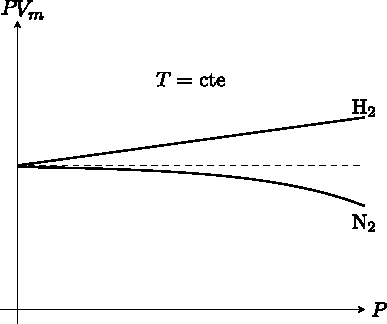
\includegraphics[width=.8\linewidth]{amagat_deuxgaz}
		\captionof{figure}{Diagramme d'\textsc{Amagat} pour deux gaz distincts à
			faible pressions.}
	\end{center}
	\tcblower
	\begin{center}
		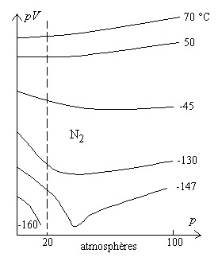
\includegraphics[width=.8\linewidth]{amagat_n2}
		\captionof{figure}{Diagramme d'\textsc{Amagat} pour le diazote à différentes
			températures.}
	\end{center}
\end{tcb}

\begin{tcbraster}[raster equal height=rows, raster columns=3]
	\begin{tcb*}[raster multicolumn=2](defi){Diagramme de \textsc{Clapeyron}}
		On appelle \textbf{diagramme de \textsc{Clapeyron}} les diagrammes $(P,V)$,
		c'est-à-dire dans lequel on représente la pression en ordonnée et le volume en
		abscisse, à température constante~: si le gaz est \textbf{parfait}, alors
		l'isotherme $T_0$ est une \textbf{parabole} d'ordonnée $y = nRT_0/V$~:
		\[
			(P)\ind{G.P.} = \frac{nRT_0}{V}
		\]
	\end{tcb*}
	\begin{tcb}(exem)<rgtt>'r'{}
		\begin{center}
			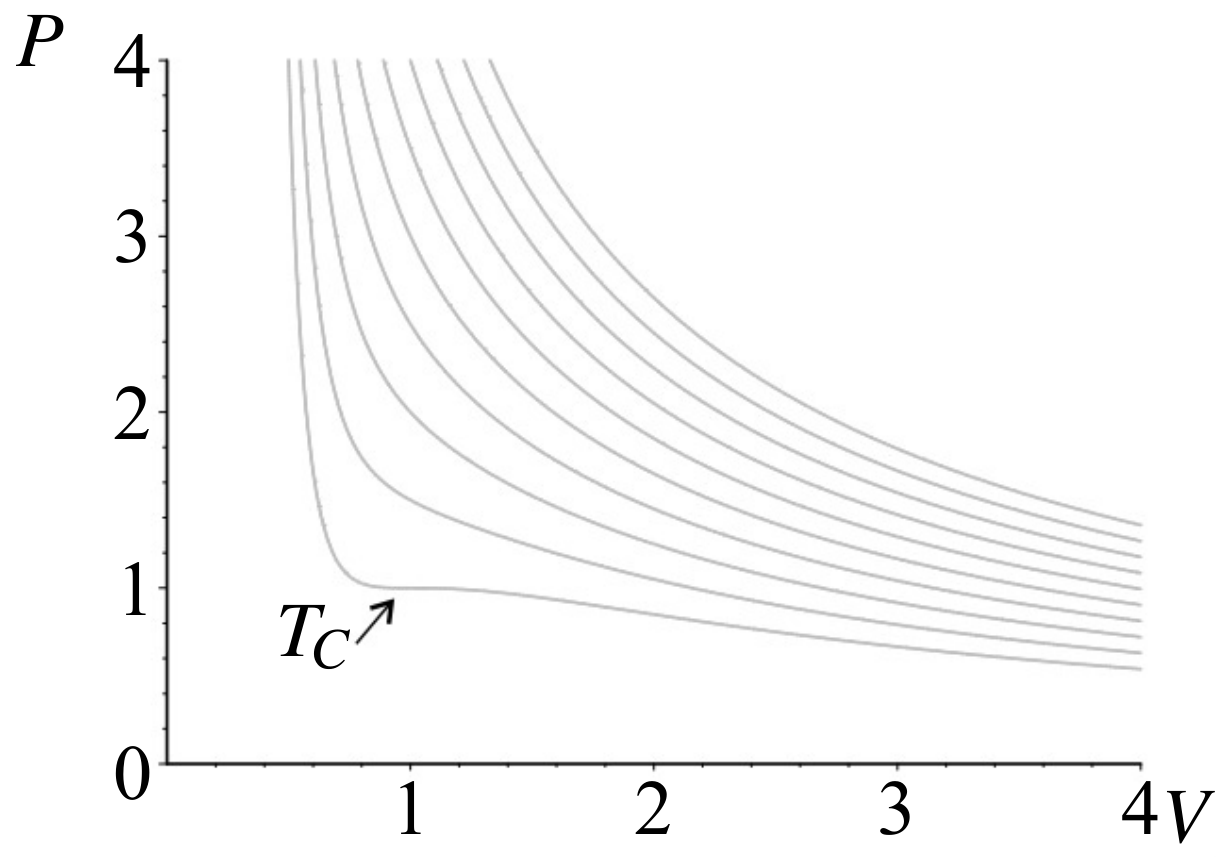
\includegraphics[width=\linewidth]{clap_intro}
			\captionsetup{justification=centering}
			\captionof{figure}{\\Isotherme réelles en $(P,V)$.}
		\end{center}
	\end{tcb}
\end{tcbraster}

\begin{tcb*}(ror){Validité du gaz parfait}
	\begin{itemize}
		\item Il existe un écart entre la courbe réelle et la courbe du gaz parfait,
		      et cet écart dépend de la température~;

		\item L'allure précise diffère d'un gaz à l'autre, mais toutes les courbes
		      d'\textbf{Amagat} de différents gaz à même température se regroupent à
		      basse pression~;
	\end{itemize}
	\bigbreak
	Ainsi, le modèle du gaz parfait est valide à faible pression et haute
	température~:
	\psw{%
		\[
			\boxed{P \ll P\ind{critique}}
			\qqet
			\boxed{T \gg T\ind{critique}}
		\]
	}%
	\vspace{-15pt}
\end{tcb*}

\begin{tcb}(rema)<lftt>{}
	À de plus fortes pressions, on utilise l'équation d'état de
	\textsc{Van Der Waals}~:
	\[
		\left( P + \frac{an^2}{V^2} \right) (V-nb) = nRT
	\]
	prenant en compte la taille des molécules (\textit{via} $b$) et
	les forces d'attraction entre elles (\textit{via} $a$).
\end{tcb}

\subsection{Énergétique}
\subsubsection{Énergie interne}

\begin{tcb*}(defi){Température cinétique}
	La température T d'un gaz parfait monoatomique est une mesure macroscopique de
	l'agitation des molécules selon \textbf{tous leurs degrés de liberté} $D$~:
	\psw{%
		\[
			\boxed{\moy{e_{c,i}} = D \times \frac{1}{2}k_B T}
		\]
	}%
	avec $D$ le nombre de degrés de liberté, et $k_B$ la \textbf{constante de
		\textsc{Boltzmann}}~: \xul{\psw{$k_B = \SI{1.3806e-23}{J.K^{-1}}$}}
\end{tcb*}

\begin{tcb*}(appl)<lftt>{$\moy{e_{c,i}}$ gaz mono- et diatomique}
	Déterminer les degrés de liberté puis l'énergie cinétique microscopique
	moyenne d'un gaz~:
	\begin{tasks}[label=\arabic*)](2)
		\task monoatomique~;
		\task diatomique rigide.
	\end{tasks}
	\tcblower
	\begin{enumerate}
		\item gaz monoatomique~:
		      \psw{%
			      Il n'y a que 3 degrés de liberté, ceux de translation selon $x$, $y$
			      et $z$, soit
			      \[
				      \moy{e_{c,i}} = 3 \times \frac{1}{2}k_B T
				      \quad \Ra \quad
				      e_c = \sum_{i=1}^{N} \moy{e_{c,i}}
				      \Lra
				      \boxed{e_c = \frac{3}{2} \cdot Nk_B \cdot T}
			      \]
		      }%
		      \vspace{-15pt}
		\item gaz diatomique rigide~:
		      \psw{%
			      Il y a trois degrés de libertés de translation, et \textbf{deux
				      degrés de rotation}~:
		      }%
		      \vspace*{-15pt}
		      \begin{center}
			      \sswitch{
				      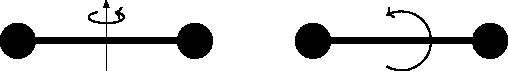
\includegraphics[scale=1, draft=true]{deglib_dia}
			      }{
				      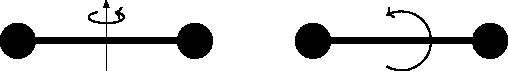
\includegraphics[scale=1]{deglib_dia}
			      }
			      \captionof{figure}{Degrés de libertés gaz diatomique.}
		      \end{center}
		      \vspace{-15pt}
		      \psw{%
			      \[
				      \moy{e_{c,i}} = (3+2) \times \frac{1}{2}k_BT
				      \quad \Ra \quad
				      e_c = \sum_{i=1}^{N} \moy{e_{c,i}}
				      \Lra
				      \boxed{e_c = \frac{5}{2} \cdot Nk_B \cdot T}
			      \]
		      }%
	\end{enumerate}
	\vspace{-15pt}
\end{tcb*}
\vspace{-10pt}
\begin{tcbraster}[raster equal height=rows, raster columns=2]
	\begin{tcb*}(prop){$U\ind{G.P.}$}
		Puisqu'il n'existe aucune interaction entre les molécules, la seule source
		d'énergie possible est leur \textbf{énergie cinétique}~:
		\psw{%
			\[
				U = e_c + \underbracket[1pt]{e_p}_{=0}
				\Lra
				\boxed{U = \frac{D}{2} nRT}
				\quad
				R = k_B \Nc_A
			\]
		}%
		\vspace{-15pt}
	\end{tcb*}
	\begin{tcb*}(demo)'r'{$U\ind{G.P.}$}
		\psw{%
			\begin{gather*}
				U = e_c = N \moy{e_{c,i}} = \frac{D}{2} \cdot Nk_B T,
				\quad
				N = n \Nc_A
				\\\Ra
				U = \frac{D}{2} \times n \underbracket{\Nc_Ak_B}_{=R} T = \frac{D}{2}nRT
				\qed
			\end{gather*}
		}%
		\vspace{-15pt}
	\end{tcb*}
\end{tcbraster}

\begin{tcb*}[sidebyside](ror){$U\ind{mono}$ et $U\ind{dia}$}
	\tcbsubtitle{\fatbox{\textbf{Gaz parfait monoatomique}}}
	\psw{%
		\[
			U\ind{mono} = \frac{3}{2}nRT
		\]
	}%
	\vspace{-15pt}
	\tcblower
	\tcbsubtitle{\fatbox{\textbf{Gaz parfait diatomique}}}
	\psw{
		\[
			U\ind{dia} = \frac{5}{2}nRT
		\]
	}
	\vspace{-15pt}
\end{tcb*}

\begin{tcb}(rema)<lftt>{Énergie interne d'un gaz parfait}
	\begin{itemize}
		\item $U$ est bien une grandeur \textbf{extensive}, puisque
		      \textbf{proportionnelle à $n$}.
		\item L'énergie interne molaire d'un gaz parfait ne dépend \textbf{que de la
			      température}~:
		      \psw{%
			      \[
				      U_m = \frac{U}{n} = \frac{D}{2}RT
				      \Lra
				      \boxed{U_m = U_m(T)}
			      \]
		      }%
		      \vspace{-15pt}
	\end{itemize}
\end{tcb}

\subsubsection{Capacité thermique}
En appliquant la définition~\ref{defi:cv}, on trouve
\begin{tcb*}[sidebyside](ror){$C_V$ du gaz parfait}
	\tcbsubtitle{\fatbox{\textbf{Gaz parfait monoatomique}}}
	\psw{%
		\[
			C_{V} = \frac{3}{2}nR
			\Lra
			C_{V,m} = \frac{3}{2}R
		\]
	}%
	\vspace{-15pt}
	\tcblower
	\tcbsubtitle{\fatbox{\textbf{Gaz parfait diatomique}}}
	\psw{
		\[
			C_V = \frac{5}{2}nRT
			\Lra
			C_{V,m} = \frac{5}{2}R
		\]
	}
	\vspace{-15pt}
\end{tcb*}

\begin{tcb}[breakable](appl)<lftt>{Capacité thermique de l'air}
	L'air est composé à 78\% de diazote, 21\% de dioxygène et 1\% d'argon.
	Calculer sa capacité thermique molaire. Comparer à la capacité thermique
	molaire d'un gaz purement diatomique et conclure.
	\tcblower
	\psw{%
		$C_V$ étant extensive, on peut sommer les $C_V$ des gaz individuels~:
		\begin{gather*}
			C_V =
			\num{0.78}n \times \frac{5}{2}R +
			\num{0.21}n \times \frac{5}{2}R +
			\num{0.01}n \times \frac{3}{2}R
			\\\Ra
			C_{V,m} =
			\num{0.78} \times \frac{5}{2}R +
			\num{0.21} \times \frac{5}{2}R +
			\num{0.01} \times \frac{3}{2}R
			\\\Ra
			\xul{C_{V,m} = \SI{20.70}{J.K^{-1}.mol^{-1}}}
			\approx \SI{20.79}{J.K^{-1}.mol^{-1}}
		\end{gather*}
		D'un point de vue thermodynamique, on peut considérer l'air comme un gaz
		parfait diatomique.
	}%
	\vspace{-20pt}
\end{tcb}

\subsection{Vitesse}
\begin{tcb*}[breakable](prop){Distribution des vitesses}
	\noindent
	\begin{minipage}[c]{.57\linewidth}
		En observant un gaz, que ce soit micro- ou macroscopiquement,
		\begin{itemize}
			\item Aucune direction n'est privilégiée~;
			\item L'observation ne dépend pas du lieu choisi.
		\end{itemize}
		On dit qu'il y a~:
	\end{minipage}
	\begin{minipage}[c]{.40\linewidth}
		\begin{center}
			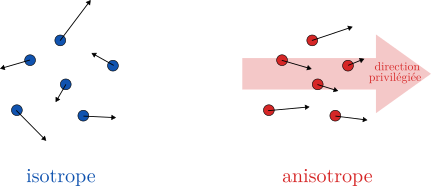
\includegraphics[width=\linewidth]{vitesse_iso}
		\end{center}
	\end{minipage}
	\begin{itemize}
		\bitem{Isotropie}~: \psw{les vitesses sont orientées dans toutes les
			directions, de manière aléatoire et uniforme~;}
		\bitem{Homogénéité}~: \psw{leur répartition est la même en tout point de
			l'espace.}
	\end{itemize}
\end{tcb*}

On observe alors une répartition suivant une densité de probabilité de la
forme~:
\begin{center}
	\sswitch{
		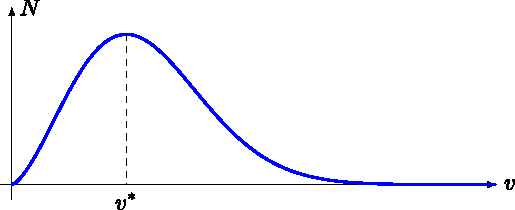
\includegraphics[width=.6\linewidth, draft=true]{distrib_gaz}
	}{
		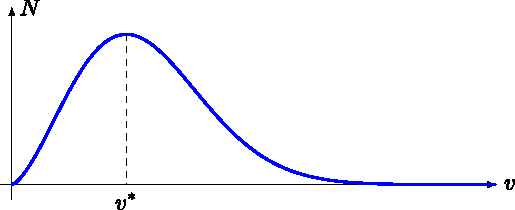
\includegraphics[width=.6\linewidth]{distrib_gaz}
	}
	\captionof{figure}{Distribution des vitesses dans un gaz.}
\end{center}

Ainsi, la \textbf{vitesse vectorielle moyenne} est nulle (par isotropie), mais
on note une valeur de vitesse scalaire de plus haute probabilité que les autres,
qui va nous servir pour décrire tout le gaz~:

\begin{tcb*}(prop){Vitesse quadratique moyenne}
	De l'étude énergétique d'un gaz et des propriétés de la distribution de
	vitesse, on en déduit la \textbf{vitesse quadratique moyenne} des molécules
	d'un gaz monoatomique~:
	\psw{%
		\[
			\setlength{\fboxsep}{3mm}
			\boxed{v^* = \sqrt{\moy{v^2}} = \sqrt{\frac{3RT}{M}}}
		\]
	}%
\end{tcb*}
\begin{tcb*}(demo){Vitesse quadratique moyenne}
	\begin{DispWithArrows*}[format=LrCL, fleqn, mathindent=0pt]
		\text{D'une part~:} &
		\psw{\moy{e_{c,i}}}
		&=&
		\psw{\frac{3}{2}k_B T}
		\\
		\text{D'autre part~:} &
		\psw{\moy{e_{c,i}} = \moy{\frac{1}{2}mv^2}}
		&=&
		\psw{\frac{1}{2}m{v^*}^2}
		\Arrow{$\times N = n\Nc_A$}
		\\
		\text{Pour l'ensemble~:} &
		\hspace{100pt}
		\psw{\frac{1}{2}n \underbracket[1pt]{m\Nc_A}_{=M} {v^*}^2}
		&=&
		\psw{\frac{3}{2}n \underbracket[1pt]{\Nc_a k_B}_{=R} T}
		\\
		& \Lra
		\psw{\frac{1}{2}M {v^*}^2}
		&=&
		\psw{\frac{3}{2}RT}
		\qed
	\end{DispWithArrows*}
\end{tcb*}

\begin{tcb}(odgr)<lftt>{$v^*$}
	Calculez $v^*$ pour~:
	\begin{tasks}[label=\arabic*)](2)
		\task L'air à \SI{25}{\degreeCelsius}~;
		\task L'air à \SI{0}{\degreeCelsius}~;
	\end{tasks}
	\tcblower
	\begin{isd}
		\psw{    \[
				\left\{
				\begin{array}{rcl}
					T & = & \SI{300}{K}
					\\
					M & = & \SI{29}{g.mol^{-1}}
				\end{array}
				\right.
				\Ra
				\xul{
					v^* \approx \SI{500}{m.s^{-1}}
				}
			\]}
		\tcblower
		\psw{    \[
				\left\{
				\begin{array}{rcl}
					T & = & \SI{273}{K}
					\\
					M & = & \SI{29}{g.mol^{-1}}
				\end{array}
				\right.
				\Ra
				\xul{
					v^* \approx \SI{480}{m.s^{-1}}
				}
			\]}
	\end{isd}
\end{tcb}

\section{Phases condensées}
\subsection{Modélisation}
\begin{tcb*}(defi){Phase condensée}
	On dit qu'une phas est \textbf{condensée} lorsqu'elle possède une
	\textbf{grande masse molaire} (ou volumique), ce qui implique qu'elle occupe
	un volume défini. On dit de plus qu'elle est~:
	\smallbreak
	\begin{isd}
		\tcbsubtitle{\fatbox{\textbf{Incompressible}}}
		\psw{Son volume ne dépend pas de la pression~:
			\[
				\eval{\pdv{V}{P}}_{n,T} = 0
			\]
		}
		\vspace{-15pt}
		\tcblower
		\tcbsubtitle{\fatbox{\textbf{Indilatable}}}
		\psw{Son volume ne dépend pas de la température~:
			\[
				\eval{\pdv{V}{T}}_{n,P} = 0
			\]
		}
		\vspace{-15pt}
	\end{isd}
	Autrement dit, une phase \textbf{incompressible et indilatable} de quantité de
	matière $n$ fixée \textbf{ne peut changer de volume}.
\end{tcb*}

\subsection{Équation d'état}
\begin{tcb*}(prop){Équation d'état phase condensée}
	Elle se déduit de sa définition de la phase~: le volume ne dépend que de la
	quantité de matière, soit
	\psw{%
		\[
			\boxed{\frac{V}{n} = \cte}
		\]
	}%
	\vspace{-15pt}
\end{tcb*}

\begin{tcb}(rema)<lftt>{}
	Si on prend en compte le fait que le volume change un peu avec la pression et
	la température, on peut écrire
	\[
		\frac{V}{n} = V_{m,0} \left( 1 + \alpha_{P} (T-T_0) + \chi_T (P-P_0)\right)
	\]
	avec $\chi_T = -\frac{1}{V} \eval{\pdv{V}{P}}_{T,n}$ la compressibilité
	isotherme, et $\alpha_P = \frac{1}{V} \eval{\pdv{V}{T}}_{P,n}$ la dilatation
	thermique.
\end{tcb}

\begin{tcb}(odgr)<lftt>{Comparaison aux gaz}
	\begin{center}
		\captionof{table}{Évolution relative de volume pour une même variation selon
			la phase.}
		\begin{tabularx}{.7\linewidth}{cYYYY}
			\toprule
			                         &                           &            & \multicolumn{2}{c}{$\dd{V}/V$}
			\\
			\cmidrule(lr){4-5}
			Phase                    &
			$\alpha_P~(\si{K^{-1}})$ & $\chi_T~(\si{bar^{-1}})$  &
			$\Delta{T} = \SI{10}{K}$ & $\Delta{P} = \SI{1}{bar}$
			\\
			\midrule
			Eau                      & \num{2.0e-4}              & \num{5e-5} & \num{0.2}\%                    & \num{0.005}\%
			\\
			Gaz                      & \num{3e-3}                & \num{1}    & \num{3}\%                      & \num{100}\%
			\\
			\bottomrule
		\end{tabularx}
	\end{center}
	% \begin{itemize}
	%   \item Pour l'eau liquide à pression et température ambiantes,
	% \[
	%   V_{m,0} = \frac{M_{\ce{H_2O}}}{\rho_0} = \SI{18}{mL.mol^{-1}}
	%   \qqav
	%   \alpha_P = \SI{1.8e-4}{K^{-1}}
	%   \qet
	%   \chi_T = \SI{5e-5}{bar^{-1}}
	% \]
	%   \item Pour un gaz dans les mêmes conditions, on trouve $\chi_T =
	%     \SI{1}{bar^{-1}}$ et $\alpha_P = \SI{3e-3}{K^{-1}}$, soit une variation de
	%     $\dd{V}/V = \num{3}\%$
	% \end{itemize}
\end{tcb}

\subsection{Énergétique}

\subsubsection{Énergie interne}
\begin{tcbraster}[raster equal height=rows, raster columns=2]
	\begin{tcb*}(prop){$U\ind{cond}$}
		Comme pour le G.P., l'énergie interne molaire d'une phase condensée
		incompressible et indilatable \textbf{ne dépend que de la température}~:
		\psw{%
			\[
				\boxed{U_m\sup{cond} = \frac{U}{n} = U_m(T)}
			\]
		}%
	\end{tcb*}
	\begin{tcb*}(demo)'r'{$U\ind{cond}$}
		Ne pouvant changer de volume, son énergie ne peut déjà dépendre que de $n$ et
		$T$~:
		\psw{
			\[
				U = U(n,T)
			\]}%
		Or, l'énergie interne est extensive, donc proportionnelle à $n$, soit
		\psw{%
			\[
				U(n,T) = nU_m(T)
				\qed
			\]
		}%
		\vspace{-15pt}
	\end{tcb*}
\end{tcbraster}

\subsubsection{Capacité thermique}
\begin{tcb*}(prop){$C\ind{cond}$}
	Par définition, la proportionnalité entre $U$ et $T$ est la capacité
	thermique~:
	\psw{%
		\[
			C_{V,m}\sup{cond} = \dv{U_m\sup{cond}}{T}
			\Lra
			\boxed{U_m\sup{cond} = C_{V,m}\sup{cond}T}
		\]
	}%
\end{tcb*}

\begin{tcb}(odgr)<lftt>{Capacités thermiques phases condensées}
	\begin{center}
		\begin{tabular}{cccccc}
			\toprule
			\textbf{Élément}                  &
			Eau\ftn{À connaître absolument~!} & Bois                  & Fer       & Aluminium & Cuivre
			\\
			$c$~(\si{J.K^{-1}.kg^{-1}})       &
			\num{4180}                        & \numrange{1000}{2000} & \num{444} & \num{897} & \num{385}
			\\
			\bottomrule
		\end{tabular}
	\end{center}
\end{tcb}


\end{document}
